\chapter{Einrichtung einer Ultra-Low-Latency Videoübertragung \label{sec:webrtc}}
\section{Anforderungen an die Videoübertragung (Jürgens)}
Die angebundene Kamera des RPi5 soll zukünftig neben dem Stream für die KI-Auswertung auch das 'Auge' des Roboters darstellen. So soll die Sicht des Roboters in nahezu Echtzeit abrufbar sein. Daher muss neben einer robusten Verbindung besonders auch die Latenz der Videoübertragung so gering wie möglich gehalten werden. Die bisherige Implementation mittels einer libcamera-Pipeline als Sender und einer GStreamer-Pipeline als Empfänger ist mit einer Latenz von etwa 1 Sekunde nicht für die Echtzeitübertragung geeignet. Nach einer Recherche zu verschiedenen Streaming-Protokollen und -Techniken wurde die Entscheidung getroffen, dass zukünftig eine Lösung mittels WebRTC verwendet werden soll. WebRTC bietet eine Lösung mit einer Latenz von unter 500 ms an, welches für dieses Projekt mehr als ausreichend ist \cite{WebRTCLatency}.

\section{Grundlegende Informationen zu WebRTC (Jürgens)}
WebRTC ist ein freies, offenes Softwareprojekt welches eine Lösung für die Echtzeitkommunikation von Browsern und mobilen Anwendungen bietet. Mittels einer Peer-To-Peer Verbindung können unter Anderem Audio- und Videodaten in Echtzeit zwischen den Peers übertragen werden. Dieses Vorgehen ermöglicht eine direkte Kommunikation zwischen den Peers ohne einen zentralen Server, was zu einer geringeren Latenz führt.
Bei dem Verbindungsaufbau wirken verschiedene Komponenten und Protokolle zusammen, um eine stabile und sichere Verbindung zwischen den Peers herzustellen. Ein wichtiger Bestandteil von WebRTC ist der Signalisierungsprozess. Dieser ist für den Austausch von Metadaten zwischen den Peers verantwortlich. \cite{WebRTCBasics}

\section{Herstellung der WebRTC-Verbindung (Jürgens)}
Insgesamt wurden zwei Ansätze bei der Herstellung der WebRTC-Verbindung zwischen dem RPI5 und dem Laborrechner verfolgt. Der erste Ansatz war der direkte Aufbau einer Peer-To-Peer Verbindung.
Mit der Python-Bibliothek \texttt{aiortc} konnte eine WebRTC-Verbindung hergestellt werden. Mittels GStreamer und OpenCV wird diese Verbindung mit dem Kamerabild angereichert und an den Empfänger gesendet. Durch das Hinzufügen eines Keep-Alives-Kanal wird sichergestellt, dass die Verbindung zwischen den Peers beibehalten wird und nicht nach einer gewissen Zeit abbricht. Mit diesem Ansatz konnte eine stabile Verbindung mit geringer Latenz zwischen dem RPi5 und dem Laborrechner hergstellt werden.

Durch weitere Absprachen mit dem Team kam der Wunsch auf, dass die Videoübertragung nicht nur einzig und allein für die KI-Auswertung genutzt werden soll, sondern auch aus dem LAN über eine Website aufrufbar sein soll. Mit dieser Anforderung wurde der zweite Ansatz verfolgt, welcher den Einsatz eines MediaMTX-Servers beinhaltet. MediaMTX ist ein Open-Source Media-Server welcher eine Vielzahl von Protokollen unterstützt, darunter auch WebRTC. Der MediaMTX-Server wird dabei auf dem RPI5 installiert und ausgeführt. Die Konfiguration der Servers erfolt über eine YML-Datei.
In dieser können beispielsweise Ports und Protokolle festgelegt werden. Neben der grundlegenden Konfiguration kann hier auch das Startverhalten des Servers festgelegt werden. So wird beim Start automatisch ein Libcamera-Stream an den Server mittels RTSP übergeben. Über den Standardport 8889 kann der Stream schlussendlich über WebRTC mittels Browser abgerufen werden. Um den WebRTC-Stream auch außerhalb einer Browser-Umgebung abrufen zu können, bietet MediaMTX eine WHEP-Schnittstelle an. Über diese WHEP-Schnittstelle kann der Stream beispielsweise in anderen Anwendungen abgerufen werden. Diese Schnittstelle ermöglicht es, den Stream in unserem Python-Script zu verwenden und die KI-Auswertung auf dem Stream durchzuführen. 

Mit dieser Implementation ist es möglich die KI-Auswertung auf einem Ultra-Low-Latency Stream anzuwenden und so in nahezu Echtzeit die Objekterkennung durchzuführen während der Kamerastream von anderen Geräten aus dem LAN per Browser angeschaut werden kann. In der Abbildung \ref{fig:KI-webRTC-Architektur} ist die Architektur des WebRTC-Streams in Zusammenarbeit mit der KI-Auswertung noch einmal dargestellt. 

\begin{figure}[H]
  \centering
  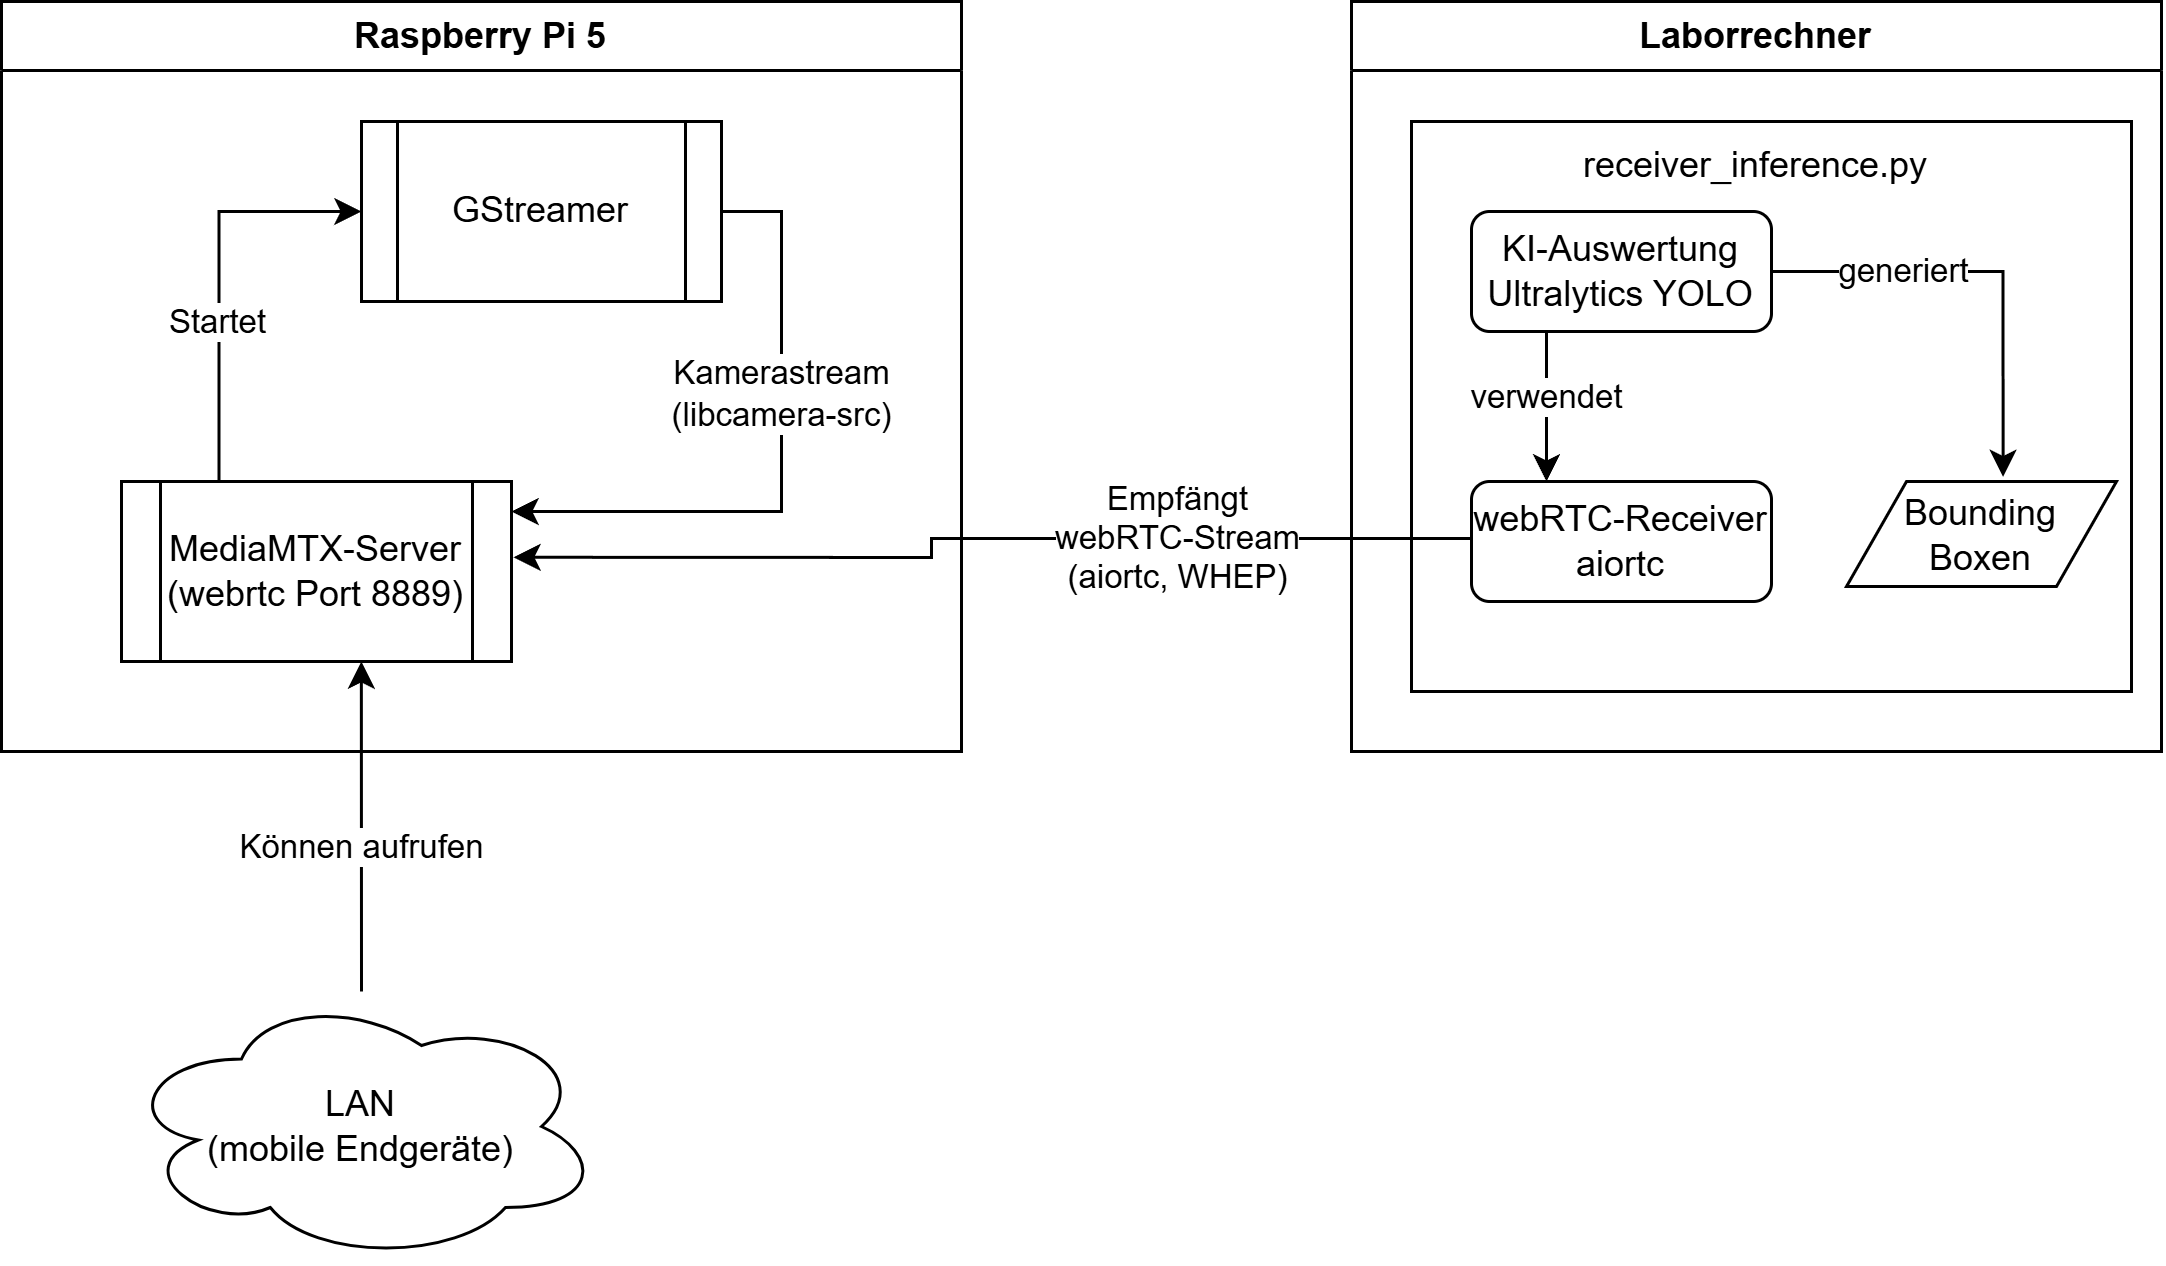
\includegraphics[width=0.95\textwidth]{images/ki-webrtc-arch.png}
  \caption{Architekturübersicht: Zusammenspiel von KI-Modell und WebRTC-Streaming}
  \label{fig:KI-webRTC-Architektur}
\end{figure}
